% This is samplepaper.tex, a sample chapter demonstrating the
% LLNCS macro package for Springer Computer Science proceedings;
% Version 2.20 of 2017/10/04
%
\documentclass[runningheads]{llncs}
%
\usepackage{graphicx}
\usepackage{booktabs}
\usepackage{adjustbox}
\usepackage{tabularx}
\usepackage{titlesec}
\usepackage{float}
% to get newline after subsubsection 
\titleformat{\subsubsection}[runin]{\normalfont\bfseries}{\thesubsubsection}{2em}{}[\\]
\usepackage[margin=1.3in]{geometry}
% Used for displaying a sample figure. If possible, figure files should
% be included in EPS format.
%
% If you use the hyperref package, please uncomment the following line
% to display URLs in blue roman font according to Springer's eBook style:
% \renewcommand\UrlFont{\color{blue}\rmfamily}

\begin{document}
%
\title{DM1\thanks{Supported by organization x.}}
%
%\titlerunning{Abbreviated paper title}
% If the paper title is too long for the running head, you can set
% an abbreviated paper title here
%
\author{Tim Mooren\inst{1}\orcidID{11710160} \and
Second Author\inst{1}\orcidID{1111-2222-3333-4444} \and
Third Author\inst{1}\orcidID{2222--3333-4444-5555}}
%
\authorrunning{F. Author et al.}
% First names are abbreviated in the running head.
% If there are more than two authors, 'et al.' is used.
%
\institute{Vrije Universiteit Amsterdam, The Netherlands}
%
\maketitle              % typeset the header of the contribution
%
\begin{abstract}
The abstract should briefly summarize the contents of the paper in
150--250 words.

\keywords{First keyword  \and Second keyword \and Another keyword.}
\end{abstract}
%
%
%
\section{Task 1: DATA PREPARATION}

\subsection{TASK 1A: EXPLORATORY DATA ANALYSIS}

\subsubsection{Data properties \& variables} 
\phantom
\smallskip

% Notice all sorts of properties of the dataset: how many records are there, how many attributes, what kinds of attributes are there, ranges of values, distribution of values, relationships between attributes, missing values, and so on. A table is often a suitable way of showing such properties of a dataset. Notice if something is interesting (to you, or in general), make sure you write it down if you find something worth mentioning.


Data was acquired in 'long form', where each row consisted of the following: a \textit{time entry}, an \textit{id}, a \textit{variable} and a \textit{value}. In total, there were 376912 entries in the dataset amassed by 27 users, of which 202 had explicitly indicated missing values (denoted 'NA'), belonging to the variables \textit{circumplex.arousal} and \textit{circumplex.valence}. \\

% many time entries 
Time entries were not consistent across variables, since the variables had a different collection methods (eg. manual input, automatic collection), meaning that certain variables were collected much more frequently and with shorter time intervals between each entry. For example, a variable such as 'screen' received many entries since an entry was created every time a user was on his phone, whereas the 'mood' variable was manually collected around 4 times a day. This discrepancy in collection methods created a dataset with very inconsistent timestamps. Indeed, of the 376913 total rows, 336907 of them were unique time entries. \\

% different variables
We can call 'time based' variables the ones that were automatically collected by user phone usage (ie. all \textit{appCat} variables), 'score based' variables the ones in which the user inputs a score (eg. \textit{mood}), and 'incidence based' variables the ones where a boolean value was automatically collected (\textit{call} \& \textit{SMS}).  \\

More details on each variable and their properties can be found in \textit{Table...} \\


+ table, when I manage to format it right... fucking latex always being super cringe
% \begin{tabular}{lrrrrrrrr}
\toprule
{} &     count &        mean &         std &        min &       25\% &        50\% &         75\% &        max \\
variable             &           &             &             &            &           &            &             &            \\
\midrule
activity             &   22965.0 &    0.115958 &    0.186946 &      0.000 &   0.00000 &   0.021739 &    0.158333 &      1.000 \\
appCat.builtin       &   91288.0 &   18.538262 &  415.989243 & -82798.871 &   2.02000 &   4.038000 &    9.922000 &  33960.246 \\
appCat.communication &   74276.0 &   43.343792 &  128.912750 &      0.006 &   5.21800 &  16.225500 &   45.475750 &   9830.777 \\
appCat.entertainment &   27125.0 &   37.576480 &  262.960476 &     -0.011 &   1.33400 &   3.391000 &   14.922000 &  32148.677 \\
appCat.finance       &     939.0 &   21.755251 &   39.218361 &      0.131 &   4.07200 &   8.026000 &   20.155000 &    355.513 \\
appCat.game          &     813.0 &  128.391615 &  327.145246 &      1.003 &  14.14800 &  43.168000 &  123.625000 &   5491.793 \\
appCat.office        &    5642.0 &   22.578892 &  449.601382 &      0.003 &   2.00400 &   3.106000 &    8.043750 &  32708.818 \\
appCat.other         &    7650.0 &   25.810839 &  112.781355 &      0.014 &   7.01900 &  10.028000 &   16.829250 &   3892.038 \\
appCat.social        &   19145.0 &   72.401906 &  261.551846 &      0.094 &   9.03000 &  28.466000 &   75.372000 &  30000.906 \\
appCat.travel        &    2846.0 &   45.730850 &  246.109307 &      0.080 &   5.08650 &  18.144000 &   47.227250 &  10452.615 \\
appCat.unknown       &     939.0 &   45.553006 &  119.400405 &      0.111 &   5.01800 &  17.190000 &   44.430500 &   2239.937 \\
appCat.utilities     &    2487.0 &   18.537552 &   60.959134 &      0.246 &   3.15850 &   8.030000 &   19.331000 &   1802.649 \\
appCat.weather       &     255.0 &   20.148714 &   24.943431 &      1.003 &   8.68400 &  15.117000 &   25.349000 &    344.863 \\
call                 &    5239.0 &    1.000000 &    0.000000 &      1.000 &   1.00000 &   1.000000 &    1.000000 &      1.000 \\
circumplex.arousal   &    5628.0 &   -0.098207 &    1.047073 &     -2.000 &  -1.00000 &   0.000000 &    1.000000 &      2.000 \\
circumplex.valence   &    5628.0 &    0.689291 &    0.661030 &     -2.000 &   0.00000 &   1.000000 &    1.000000 &      2.000 \\
mood                 &    5628.0 &    6.993870 &    1.031496 &      1.000 &   7.00000 &   7.000000 &    8.000000 &     10.000 \\
screen               &   96578.0 &   75.335206 &  253.822497 &      0.035 &   5.32225 &  20.044500 &   62.540250 &   9867.007 \\
sms                  &    1798.0 &    1.000000 &    0.000000 &      1.000 &   1.00000 &   1.000000 &    1.000000 &      1.000 \\
hour                 &  358926.0 &   14.476764 &    5.602882 &      0.000 &  11.00000 &  15.000000 &   19.000000 &     23.000 \\
day                  &  358926.0 &    2.911508 &    1.941587 &      0.000 &   1.00000 &   3.000000 &    5.000000 &      6.000 \\
\bottomrule
\end{tabular}


\subsubsection{Frequency distributions}
\phantom
\smallskip

To get an idea of the distribution of the data, each variable was plotted as a frequency distribution histogram. We can see that most of the time based variables follow roughly a power-law distribution, where the majority of the time entries are short lived, but there are a few very long ones. On the other hand, score based variables seem to be normally distributed, which makes sense for this kind of data.  It might be important to note that a normally distributed target variable (\textit{mood}) may lead to class imbalance in later models, where low and high mood score are not as well represented. We can also get a sense of the outliers depending on how high the plot values go. 

% incidence based variables only contained entries when the 1 present, blabla...



% histogram plots - TODO
\begin{figure}[h!]
    \centering
    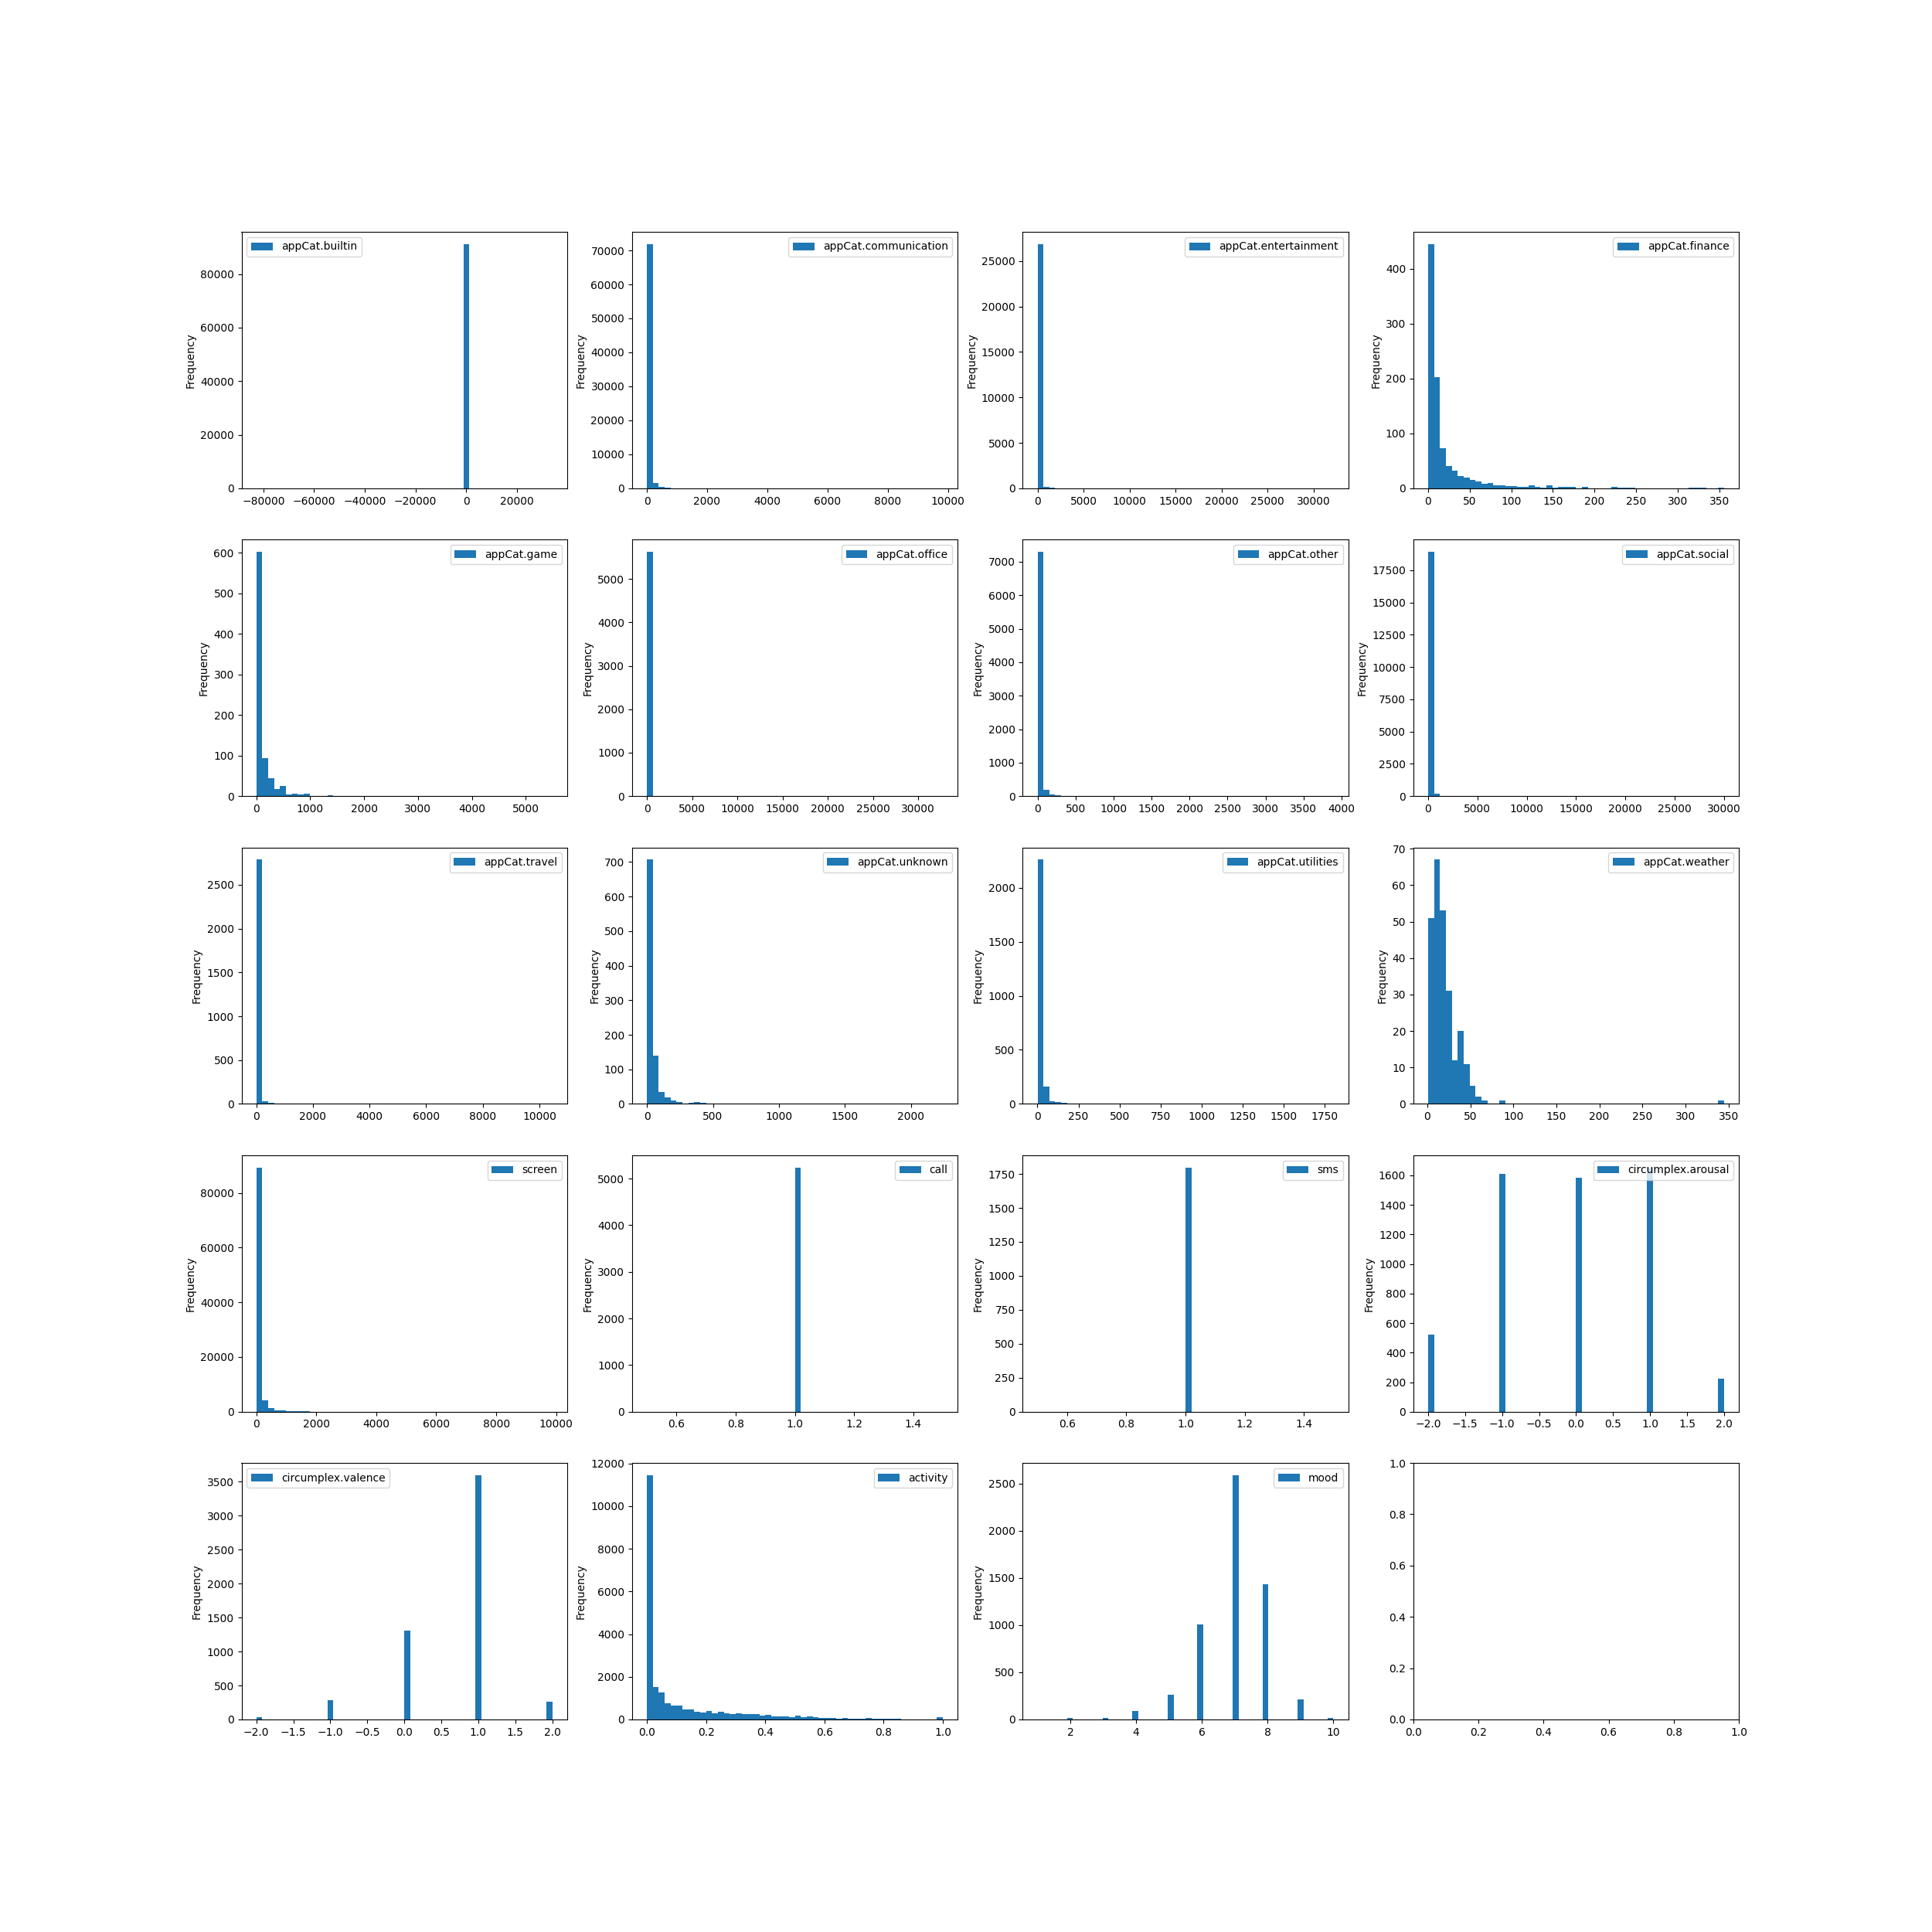
\includegraphics[width=18cm, height=18cm, trim={10cm 5cm 0 5cm}]{plots/plots_1a/distribution_plot.png}
    \caption{Caption}
    \label{fig:my_label}
\end{figure}


\subsubsection{Data trends over time}
\phantom
\smallskip

In order to get a better idea of the general time-series data trends, each variable was plotted over the (roughly) 4 month data collection period. For better visualization, the data was aggregated into days by taking the mean of all values in that day for each variable. \\

Overall, there seem to be no long term changes in \textit{mood} or any of the other predictor variables. We also see that there seem to be no clear linear or seasonal trends, but some somewhat cyclical behavior for certain variables and mostly irregular behavior for others. \\

For a lot of the time based variables (\textit{appCat} variables), the data seems to have sudden spikes in usage, with a quick return to baseline. Score variables such as \textit{mood} or \textit{circumplex} are more-so characterized by cyclical peaks and valleys. Incidence variables (\textit{Call} and \textit{SMS}) seem to drop off over time, but this could either be due to these events not occurring or these events not being recorded. \\

Additionally, we noticed that there was around a 14 day period at the start of the graphs where a large majority of variables values were missing, except for in \textit{call} and \textit{SMS}.

% time plots
\begin{figure}[h!]
    \centering
    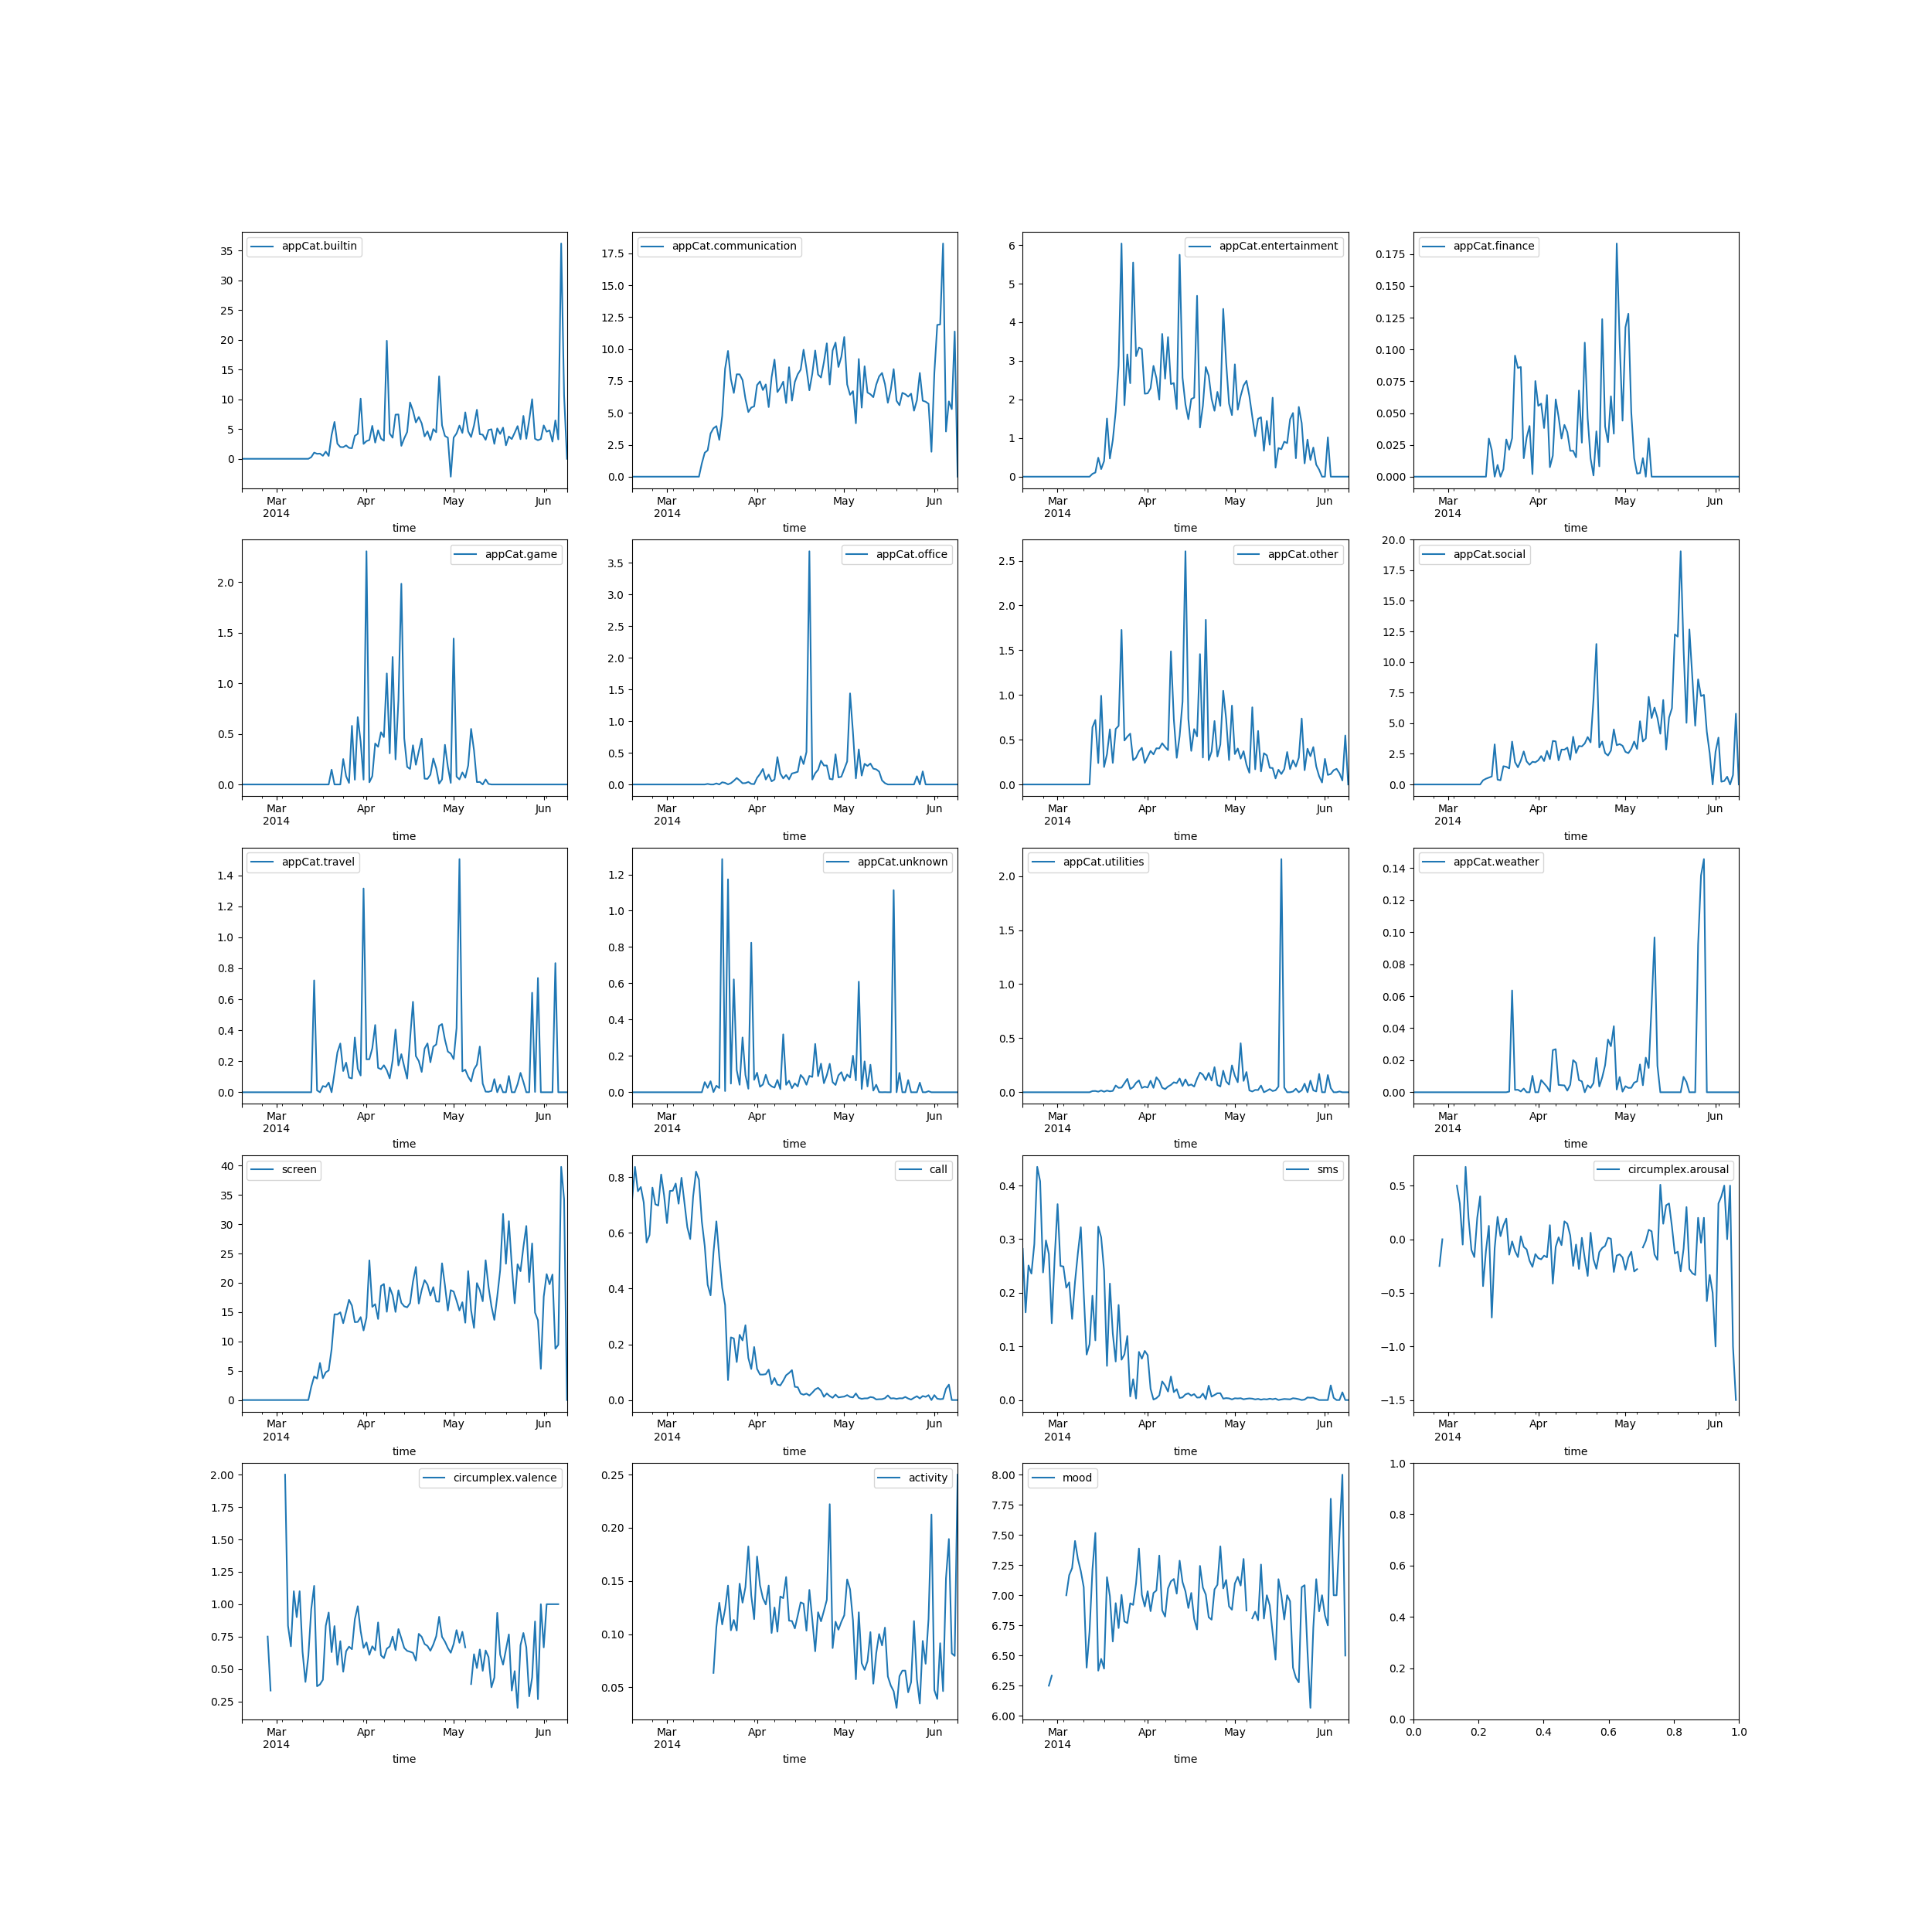
\includegraphics[width=18cm, height=18cm, trim={10cm 5cm 0 5cm}]{plots/plots_1a/time_plot.png}
    \caption{Caption}
    \label{fig:my_label}
\end{figure}



% Regarding the ranges of the values in the data, it was discovered that the variables 'appCat.builtin' and 'appCat.entertainment' had negative values, which is problematic because they represent a duration and should therefore always be positive. This was solved at the data cleaning stage.

% FALSE:? Moreover, it was discovered that the values for the variables 'sms' and 'call' are always 1 (symbolizing 'yes'). Because the values are always the same, these variables do not provide any information for our model. Thus, it was decided to omit these variables to improve efficiency of the algorithm.

% Make various plots of the data. Is there something interesting worth reporting? Report the figures, discuss what is in them. What meaning do those bars, lines, dots, etc. convey? Please select essential and interesting plots for discussion, as you have limitedspace for reporting your findings.

% 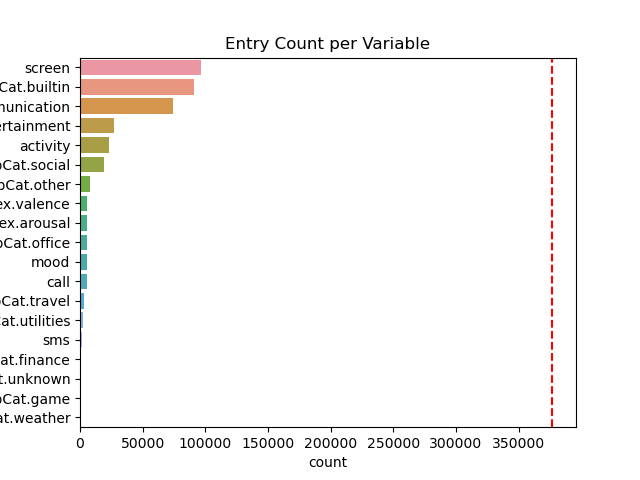
\includegraphics{plots/variable_count.png}


\subsection{TASK 1B: DATA CLEANING}

\subsubsection{Extreme and Incorrect Values} % TODO 
\phantom
\smallskip

Through the exploratory data analysis we discovered that 4 entries contained incorrect values in \textit{appCat.builtin} \& \textit{appCat.entertainment}, ie. they were negative when expected to be positive. Entries containing these values were removed from the dataset. 

\subsubsection{Data aggregation}
\phantom
\smallskip

In order for the data to be in suitable form for the later steps, the data was first put in 'wide form', where each column contained the variables and each row contained the values. Since there were so many unique time entries, this created a lot of sparsity in the dataset, where a unique timestamp for one variable meant that each of the other variables would now have empty values. \\


Because of this, all data was aggregated per day. The data was first aggregated by day and by individual ('id'), where all time based variables were aggregated with the sum, as a cumulation of the daily time allocated to that variable, and where all score based variables were aggregated with the mean, since the score isn't supposed to cumulate. \\

After this first aggregation, we noticed that there were still a lot of empty values in the dataset and decided to aggregated a second time by merging the individuals together. Since the time based variables had already been cumulated by day, we could aggregate using the mean for all variables. \\

The remaining dataset was a table containing 113 rows, where each row corresponds to a date instance with all the values for all variables after both aggregations. \\

It could have been possible not to do a second aggregation round in order to have more instances but we deemed that this would still leave too many missing values to impute, so we decided to make the trade-off in favor of having less empty values. It may also be important to note that each day is not necessarily represented equally after the aggregation, meaning that some days had a lot more values to aggregate over because of the date and method inconsistencies in the way the data was collected. \\



\subsubsection{Imputation \& removal} % TODO 
\phantom
\smallskip

The missing values from variables 'circumplex.arousal' and 'circumplex.valence' were imputed using two methods. The first method involved replacing the missing values with the mean of the variable per participant per day. It was decided to use this method rather than the overall mean because it was expected that this would result in a closer approximation to the actual value of those entries.

second method is mean per person. 


\subsection{TASK 1C: FEATURE ENGINEERING}

\subsubsection{Frequency Count}

\subsubsection{Normalization}

\subsubsection{Weekdays}
One feature that was added for the purpose of temporal mood prediction is the day of the week, which was constructed from the original data. This might be a valuable feature as it is reasonable that individual's mood may depend on the day of the week. For example, people may be in better mood on Saturday than on Monday.
\subsubsection{Participant's Average Mood}
PARTICPANT'S AVERAGE MOOD CAN BE IMPLEMENTED MAYBE?

\section{TASK 2: CLASSIFICATION }
\subsection{TASK 2A: APPLICATION OF CLASSIFICATION ALGORITHMS}

\subsection{TASK 2B: WINNING CLASSIFICATION ALGORITHMS}








\section{TASK 4: Numerical Prediction}



\section{TASK 5: EVALUATION}

\subsection{TASK 5A: CHARACTERISTICS OF EVALUATION METRICS}
% Consider the following two error measures: mean squared error (MSE) and mean absolute
% error (MAE).
% • Write down their corresponding formulae.
% • Discuss: Why would someone use one and not the other?
% • Describe an example situation (dataset, problem, algorithm perhaps) where using MSE
% or MAE would give identical results. Justify your answer (some maths may come handy, but clear explanation is also sufficient).
Mean Squared Error (MSE) and Mean Absolute Error (MAE) are two common error measures used to evaluate the performance of a model in regression tasks. The corresponding formulae for these error measures are as follows:

$$
M S E=\frac{1}{N} \sum_{i=1}^N\left(y_i-\hat{y}_i\right)^2
$$
$$
M A E=\frac{1}{N} \sum_{i=1}^N\left|y_i-\hat{y}_i\right|
$$
where $y_i$ denotes the true value of the target variable, $\hat{y}_i$ represents the predicted value of the target variable, and $N$ is the number of samples in the dataset.

A researcher might choose to use one error measure over the other based on the characteristics of the problem at hand and the desired properties of the error metric. The key differences between the two error measures are outlined below:

\textbf{Sensitivity to Outliers:} The MSE metric is more sensitive to outliers than MAE. This is because the squared term in the MSE formula magnifies the errors for large deviations. As a result, MSE tends to penalize large errors more heavily. If the researcher wants to emphasize the importance of fitting large errors correctly, they might choose MSE over MAE. Conversely, if the goal is to minimize the influence of outliers, MAE may be preferred.

\textbf{Differentiability}: MSE is a differentiable function, while MAE is not differentiable at all points due to the absolute value operation. In the context of optimization algorithms, this difference is important. Algorithms that require gradient information, such as gradient descent, benefit from using MSE since its gradient can be easily computed. On the other hand, MAE might be used with optimization algorithms that do not require gradient information.

An example situation where using MSE or MAE would yield identical results is when the errors are either all positive or all negative, with equal magnitude. For instance, consider a dataset with true target values $y = [1, 2]$ and predicted values $\hat{y} = [2, 3]$. In this case, the errors are $[-1, -1]$, and the absolute values of the errors are $[1, 1]$. Computing MSE and MAE gives:
$$
M S E=\frac{1}{2}\left((-1)^2+(-1)^2\right)=\frac{1}{2}(1+1)=1
$$
$$
M A E=\frac{1}{2}(|-1|+|-1|)=\frac{1}{2}(1+1)=1
$$




























%
% ---- Bibliography ----
%
% BibTeX users should specify bibliography style 'splncs04'.
% References will then be sorted and formatted in the correct style.
%
% \bibliographystyle{splncs04}
% \bibliography{mybibliography}
%
\begin{thebibliography}{8}
\bibitem{ref_article1}
Author, F.: Article title. Journal \textbf{2}(5), 99--110 (2016)

\bibitem{ref_lncs1}
Author, F., Author, S.: Title of a proceedings paper. In: Editor,
F., Editor, S. (eds.) CONFERENCE 2016, LNCS, vol. 9999, pp. 1--13.
Springer, Heidelberg (2016). \doi{10.10007/1234567890}

\bibitem{ref_book1}
Author, F., Author, S., Author, T.: Book title. 2nd edn. Publisher,
Location (1999)

\bibitem{ref_proc1}
Author, A.-B.: Contribution title. In: 9th International Proceedings
on Proceedings, pp. 1--2. Publisher, Location (2010)

\bibitem{ref_url1}
LNCS Homepage, \url{http://www.springer.com/lncs}. Last accessed 4
Oct 2017
\end{thebibliography}
\end{document}
